\graphicspath{{./chapters/ncov-escape/}}

\chapter{Supplementary Materials for Chapter 5}

\section{Supplementary Text}

\subsection*{Connection to phylogenetic generalized least squares}\label{ssec:pgls}

%Question: Switch i -> v, x to \lambda?

Due to shared evolutionary history among a population, the independence assumptions of regression analyses are often violated.
To address this, phylogenetic least squares (PGLS) has emerged as a way of accounting for covariance in the traits between samples from a population.
In PGLS, we assume trait values $x$ are assumed to have distribution:

\begin{equation*}
x \sim \text{Normal}(X \beta,\Sigma),
\end{equation*}
where $X$ is matrix of features, $\beta$ is the regression coefficients, and $\Sigma$ is a covariance matrix derived from a phylogenetic tree, capturing the covariance due to shared evolutionary history.

We show that our approach of modeling innovations between parent-child lineage pairs similarly captures this evolutionary structure.

When we directly model trait changes along branches using parent-child relationships, we focus on the changes $\Delta x_i = x_{\text{child}, i} - x_{\text{parent}, i}$. We assume that

\begin{equation}
\Delta x_i = Z_i \gamma + \varepsilon_i,
\end{equation}
where $Z_i$ is a vector of features for branch $i$ e.g. branch length, $\gamma$ is a vector of coefficients, and $\varepsilon_i$ is a random error term with mean 0 and variance $\sigma_i^2$.

The trait $x_i$ at node $i$ can then be written as the sum of changes from the root to that node:

\begin{align*}
    x_i &= x_{\text{root}} + \sum_{j \in \text{path to } i} (Z_j \gamma + \varepsilon_j)\\
	&= x_{\text{root}} + \left( \sum_{j \in \text{path to } i} Z_j \right) \gamma + \sum_{j \in \text{path to } i} \varepsilon_j.
\end{align*}

Simplifying it in this way allows us to easily analyze the covariance between the traits for two variants

\begin{align*}
    \Sigma_{ik} = \text{Cov}(x_i, x_k) &= \text{Cov} \left( \sum_{j \in \text{path to } i} \varepsilon_j, \sum_{l \in \text{path to } k} \varepsilon_l \right)\\
		&= \sum_{j \in \text{shared}(i, k)} \sigma_j^2.
\end{align*}

We can see that this covariance $\Sigma_{ik}$ is the sum of variances along the branches shared by nodes $i$ and $k$. 

Using our model of growth advantage innovation, we derive an expression for $x_i$ that naturally suggests an equivalent covariance matrix $\Sigma$ under PGLS.
This covariance arises directly from the cumulative variances of changes along shared evolutionary paths, providing a concrete connection between the two methods, reflect the shared evolutionary paths.


\section{Supplementary Figures}

\begin{figure}[h]
	\centering
	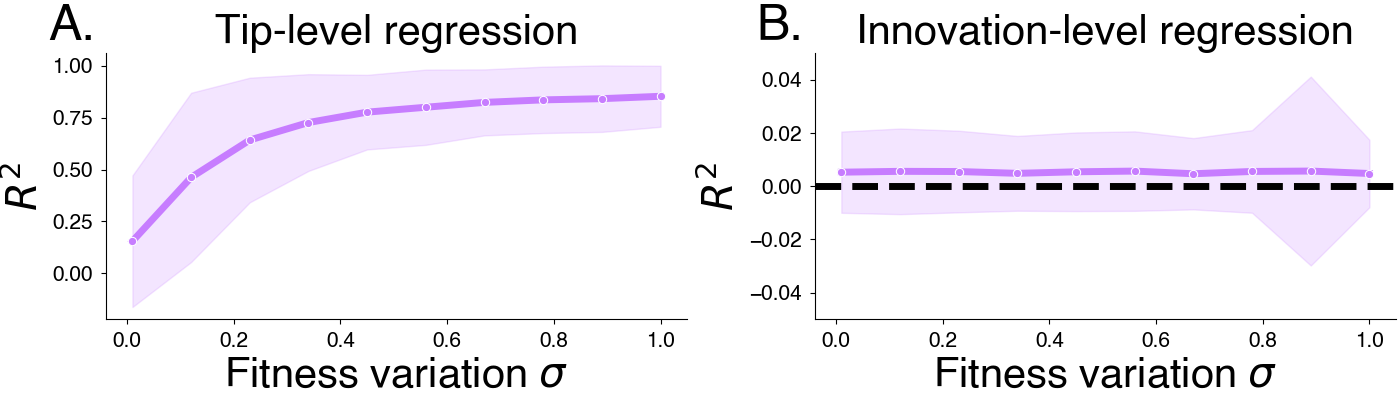
\includegraphics[width=1.0\textwidth]{./supplementary_figures/synthetic-fitness-variation-correlation.png}
	\caption{\textbf{Variance explained as a function of fitness variation.}
	    Relationship between fitness variation and the strength of regression (R²) for tip-level (A) and innovation-level (B) analyses.
	    Points represent the mean $R^2$ for each fitness variation, while the shaded regions show two standard deviations of the mean across 500 replicate simulations.
	}
	\label{fig:fitness-variation-variance-explained}
\end{figure}

\begin{figure}[h]
	\centering
	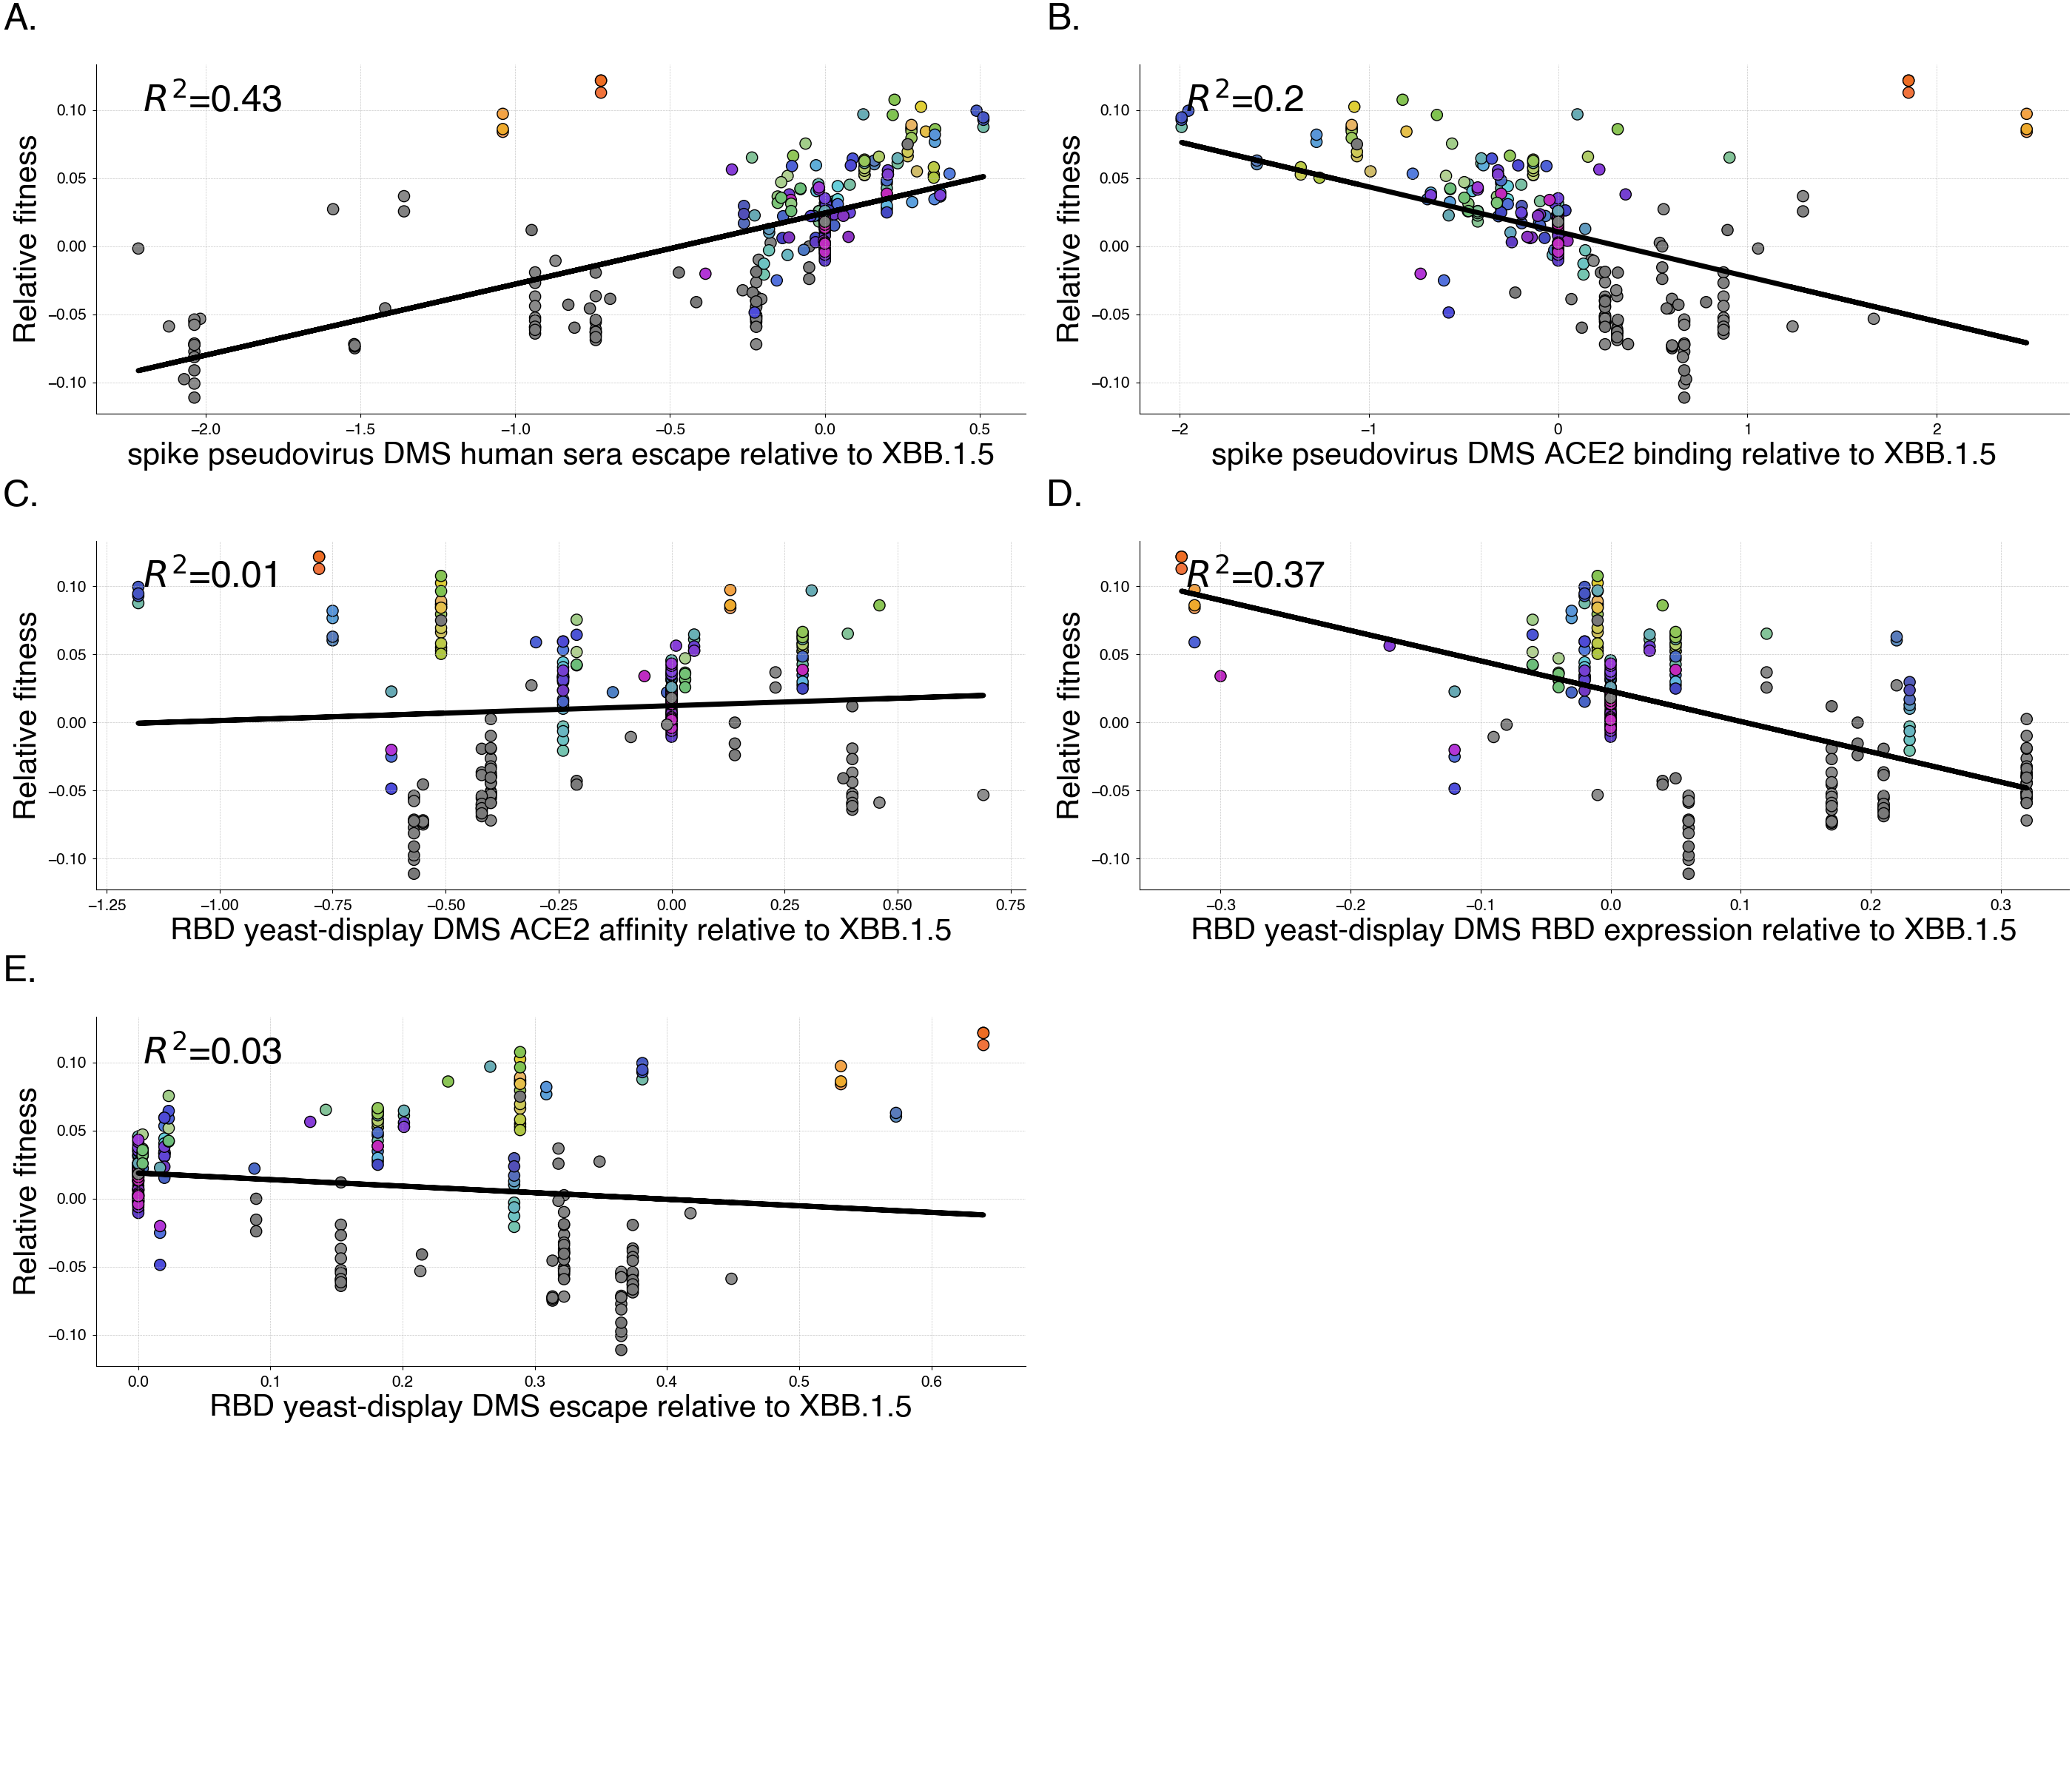
\includegraphics[width=1.0\textwidth]{./supplementary_figures/relative-fitness-single-regressions.png}
	\caption{\textbf{Naive regressions between molecular phenotypes and relative fitness}
	}
	\label{fig:relative-fitness-single-regressions}
\end{figure}


\begin{figure}[h]
	\centering
	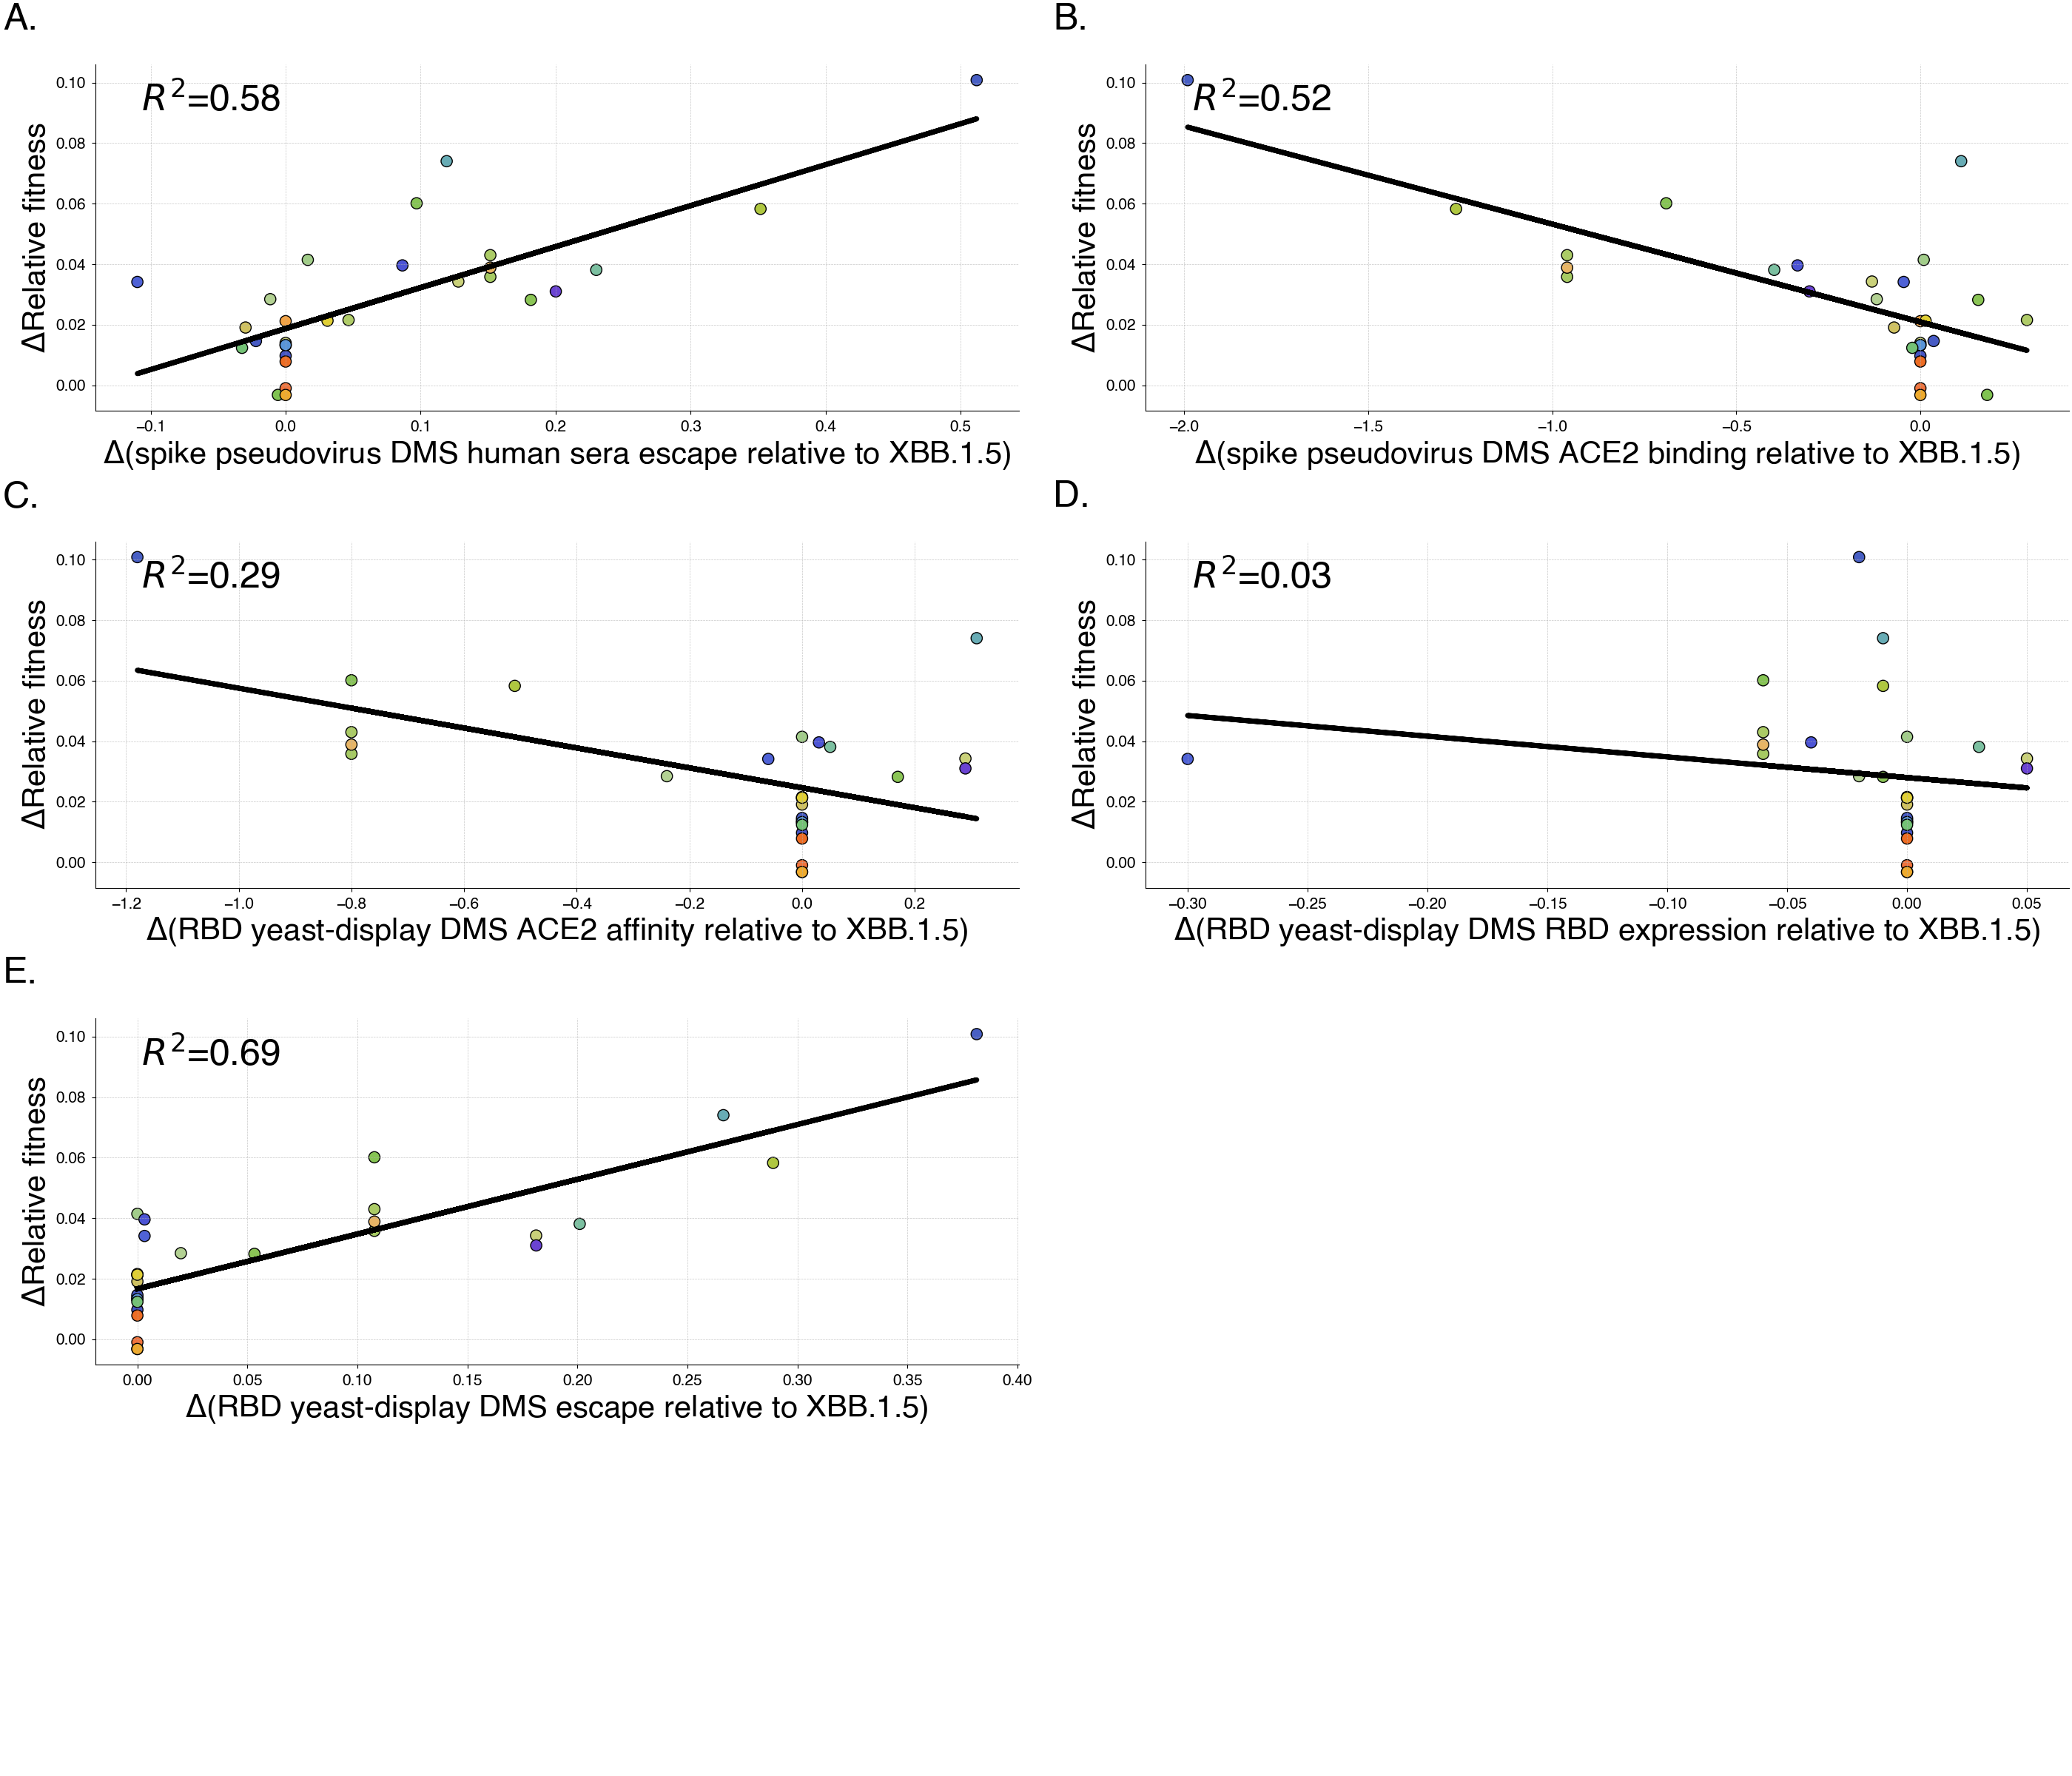
\includegraphics[width=1.0\textwidth]{./supplementary_figures/relative-fitness-innovations-single-regressions.png}
	\caption{\textbf{Innovation regressions between molecular phenotypes and relative fitness}
	}
	\label{fig:relative-fitness-innovations-single-regressions}
\end{figure}
